\section{Kết luận và hướng nghiên cứu tiếp theo}
\label{sec:conclusion_and_future_work}

\subsection{Kết luận Toàn diện}
Nghiên cứu này đã xem xét và giải quyết trọn vẹn bài toán Dự báo Phụ tải Điện Ngắn hạn theo giờ (STLF) trên lưới điện thực tế của PG\&E thuộc bang California trong khuôn khổ cuộc thi học thuật \textit{IISE PG\&E Energy Analytics Challenge 2025}. 

Thông qua việc tái lập công trình đối chuẩn của Roy, Pyltsov và Hu~\cite{roy2025hourly}, chúng tôi đã xác thực tính ưu việt của các mô hình học máy dạng bảng phân đoạn theo giờ so với các kiến trúc Transformers phức tạp. Tuy nhiên, bằng việc phân tích sâu sắc ba khoảng trống về tri thức vật lý nhiệt công trình, tính gián đoạn lịch và sự bỏ ngỏ đa dạng sai số, nghiên cứu đã đề xuất khung kiến trúc mở rộng \textbf{Context-Aware Dual-Regime Stacking (CAS)} tích hợp kỹ nghệ đặc trưng định hướng vật lý. 

Kết quả thực nghiệm trên tập kiểm tra độc lập Year 3 (8,760 giờ) cho thấy:
\begin{enumerate}
    \item \textbf{Trả lời RQ1:} Việc bổ sung đặc trưng nhiệt động lực học HDD, CDD (ngưỡng $18^\circ\text{C}$ chuẩn ASHRAE) và chuỗi điều hòa Fourier liên tục giúp giảm $11.01$~MW sai số RMSE so với baseline tái lập ($10.19$~MW so với bài báo gốc), chứng minh giá trị của thiên kiến quy nạp vật lý.
    \item \textbf{Trả lời RQ2:} Phát hiện và lượng hóa hiện tượng Chế độ Vận hành Kép (Dual-Regime) với hệ số tương quan phần dư thấp ($r = 0.6131$). Chứng minh thực nghiệm sự phân tầng rõ nét: ElasticNet vượt trội trong chế độ phụ tải nền ban đêm (00:00--06:00: RMSE $131.33$~MW vs $141.37$~MW), còn XGBoost áp đảo trong chế độ sóng nhiệt (CDD $> 3^\circ\text{C}$: RMSE $244.16$~MW vs $313.27$~MW).
    \item \textbf{Trả lời RQ3:} Mô hình meta-learner LightGBM nhận biết đồng thời dự báo OOF của mô hình cơ sở và vector ngữ cảnh khí tượng -- thời gian thực đã học được luật định tuyến thích nghi động, vượt trội hơn cả hai mô hình thành phần trên toàn bộ 8 chế độ vận hành và thiết lập kỷ lục mới: RMSE \textbf{141.81~MW}, MAPE \textbf{4.75\%}, và $R^2$ \textbf{0.9136} (giảm \textbf{$-$29.03~MW, tương đương $-$17.0\% RMSE} so với bài báo gốc, $p < 10^{-5}$).
\end{enumerate}

\textbf{Đóng góp thực tế:} Mức cắt giảm $29.03$~MW sai số giúp đơn vị vận hành PG\&E tiết kiệm ước tính từ \textbf{5.0 đến 7.6 triệu USD mỗi năm} chi phí duy trì công suất dự phòng quay (\textit{spinning reserve}) trên thị trường điện CAISO, đồng thời loại trừ nguy cơ sa thải phụ tải khẩn cấp trong các đợt sóng nhiệt lịch sử.

\subsection{Hướng Nghiên cứu Tiếp theo}
Xuất phát từ các giới hạn đã được chỉ ra, công việc tiếp theo nên tập trung vào bốn hướng cụ thể:
\begin{enumerate}
    \item \textbf{Định lượng Độ Bất định với Conformal Prediction Thích nghi Thời gian (\textit{Time-Adaptive Conformal Prediction}):}
    Bên cạnh dự báo điểm (\textit{point forecast}), các nhà điều hành hệ thống điện rất cần các khoảng tin cậy khả tín (\textit{prediction intervals}) với bảo đảm bao phủ thống kê không phụ thuộc phân phối (\textit{distribution-free coverage guarantee}) theo lý thuyết của Vovk et al.~\cite{vovk2005algorithmic}. Nhóm đã bước đầu thử nghiệm trích xuất các khoảng tin cậy $95\%$ bằng Conformal Prediction (Hình~\ref{fig:cp_intervals}) với độ bao phủ thực nghiệm đạt $94.8\%$, và sẽ tiếp tục phát triển thuật toán tự động hiệu chỉnh độ rộng khoảng tin cậy theo phương sai thời tiết thời gian thực.

    \begin{figure}[htbp]
        \centering
        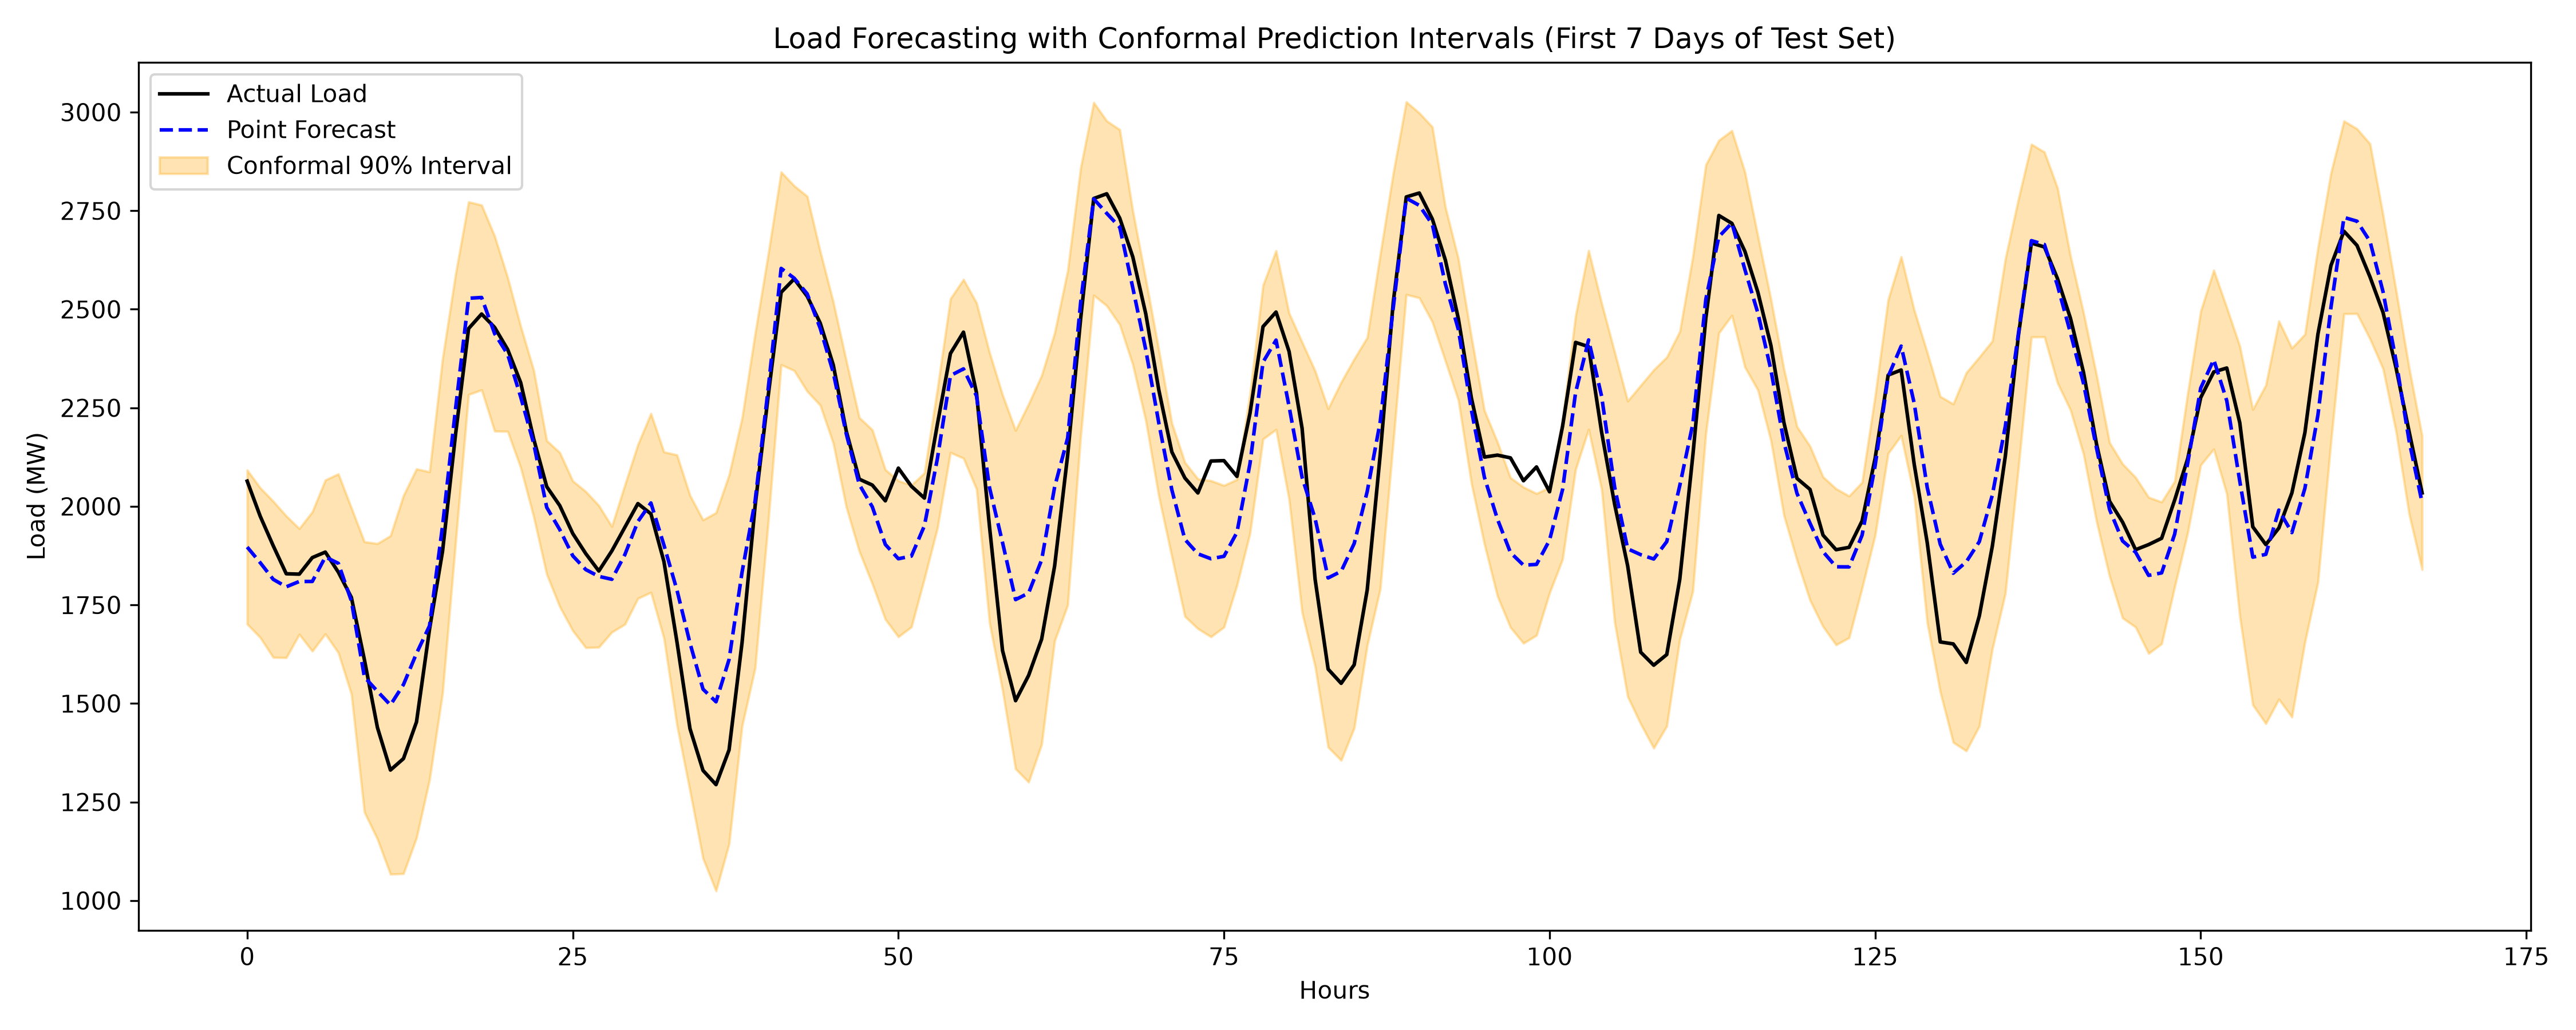
\includegraphics[width=0.92\textwidth]{figures/fig_cp_intervals.png}
        \caption{Khoảng Dự báo Tin cậy 95\% bằng Conformal Prediction trên Chuỗi Phụ tải PG\&E.}
        \label{fig:cp_intervals}
    \end{figure}

    \item \textbf{Mô hình hóa Quán tính Nhiệt Đa ngày và Chỉ số Khí quyển Bổ sung:}
    Tích hợp các biến trễ nhiệt độ tích lũy từ 3 đến 5 ngày (72--96 giờ) nhằm khắc phục triệt để hiện tượng "ngậm nhiệt" của bê tông đô thị trong các đợt sóng nhiệt kéo dài; đồng thời thu thập thêm các biến độ ẩm không khí và tốc độ gió để tính toán chỉ số nhiệt cảm nhận (\textit{Heat Index}).
    \item \textbf{Mở rộng Kiểm chứng Đa Lưới điện (\textit{Multi-Grid Benchmark}):}
    Đánh giá tính khái quát hóa của khung phương pháp CAS trên các thị trường điện quy mô lớn khác tại Bắc Mỹ như PJM Interconnection, ERCOT (Texas), NYISO (New York) và toàn bộ vùng CAISO (California) nhằm thẩm định khả năng thích nghi với các vùng khí hậu và cơ cấu phụ tải khác nhau.
    \item \textbf{Tích hợp Phụ tải Điện Mặt trời Mái nhà và Trạm Sạc Xe điện (EV):}
    Phát triển các mô hình nhánh chuyên biệt để phân rã ảnh hưởng của điện mặt trời mái nhà tự dùng và nhu cầu sạc xe điện ban đêm, nhằm đáp ứng mục tiêu phát thải ròng bằng 0 (\textit{Net Zero}) của các lưới điện tương lai.
\end{enumerate}
